\documentclass{article}
\usepackage{amsmath, fullpage}
\usepackage{graphicx}
\begin{document}

\title{Nonlinear and Quantum Optics}
%\date{\vspace{-5ex}}
\maketitle
\thispagestyle{empty}
\tableofcontents

\section{Course outline}

The planned lectures are divided into four sections:
\begin{enumerate}
    \item Heuristic linear waves: classical, semi-classical, and quantum
    \item Nonlinear response: classical, semi-classical, and quantum
    \item Zoology of nonlinear effects: Pockels (DC Kerr), harmonic generation, stimulated four-wave-mixing, spontaneous four-wave mixing
    \item Silicon micro-ring resonator example: qualitative overview, experimental results, sketch of model (self-phase modulation, cross-phase modulation, two photon absorption, stimulated four-wave mixing, free carrier dispersion, free carrier absorption, thermo-optic effect)
\end{enumerate}

Some of the processes that we are trying to cover/understand are:

\begin{itemize}
    \item Squeezing
    \item Pair generation
    \item Self- and cross-phase modulation
    \item photon distinguishability
    \item discrete and continuous variable states
    \item ...
\end{itemize}

The course will not deal with detailed circuit-level applications. Rather, the emphasis is on developing fundamental and heuristic understanding of related physics.

\subsection{System definition}
For the systems to be studied in this course, we make the following assumptions:
\begin{enumerate}
    \item no magnetic effects
    \item no metal/plasmonics
    \item no active/resonance interactions
\end{enumerate}

\begin{figure}
    \label{fig:general_system}
    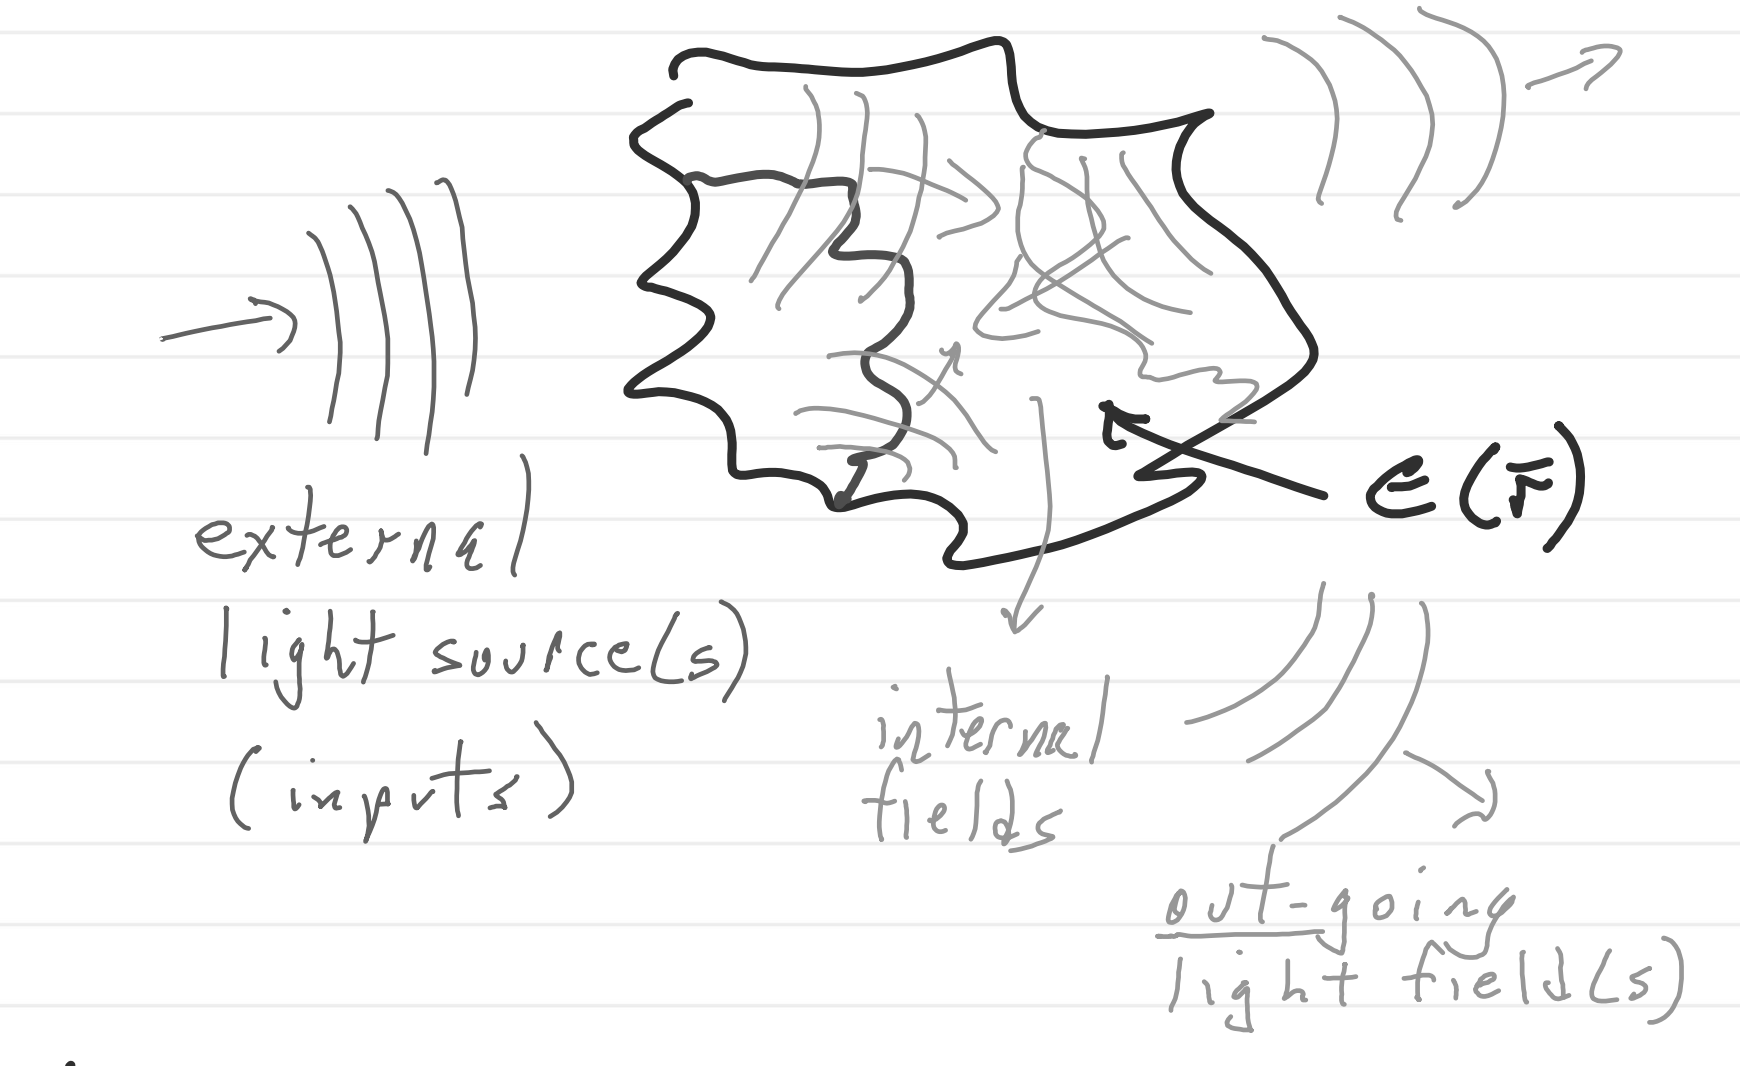
\includegraphics[width=0.6\textwidth]{figures/general_system_sketch.png}
    \centering
    \caption{h}
\end{figure}

We are fundamentally concerned with a nonlinear scattering problem, as illustrated in Figure \ref{fig:general_system}: There is an input electromagnetic field, which interacts with a dielectric environment characterized by $\epsilon(\vec{r})$, and emits out-going electromagnetic fields.

\subsection{Historical sidebar}
Nonlinear optics was historically investigated by irradiating a macroscopic nonlinear crystal with a powerful pulsed laser (Figure \ref{fig:nonlinear_crystal}). The laser is quasi-monochromatic with an angular frequency $\omega_0$, and the incoming field is 
\begin{equation}
    \vec{E}_{\rm{inc}} \sim \vec{E}_\alpha e^{i\left(\frac{\omega_0}{c}-\omega_0 t\right)},
\end{equation} 
where $\vec{E}_\alpha$ is the transverse field profile, $c$ is the speed of light, $z$ is position in the propagation direction, and $t$ is time. The crystal would emit very weak harmonics at $2\omega_0$, $3\omega_0$, and so on. The weak amplitudes of these harmonics was indicative of low conversion efficiency. 

Qualitatively, the generation of these harmonics can be understood as follows. Light is fundamentally an oscillating electromagnetic field. In a medium, this field will locally displace the charges via the Coulomb interaction. To lowest order, we can say that only the electrons are displaced, and the nuclei are stationary. A helpful analogy is to consider the electron-nucleus system to be a mass on a spring, where the spring constant is determined by the Coulomb interaction between the electron and the nucleus. At relatively low intensities, the angular frequency of the electron oscillation will be equal to that of the electromagnetic wave: $\omega_0 = \omega_{\rm{oscillation}}$. This is the linear regime. However, at high intensities, different frequency components can be excited.

\begin{figure}
    \label{fig:nonlinear_crystal}
    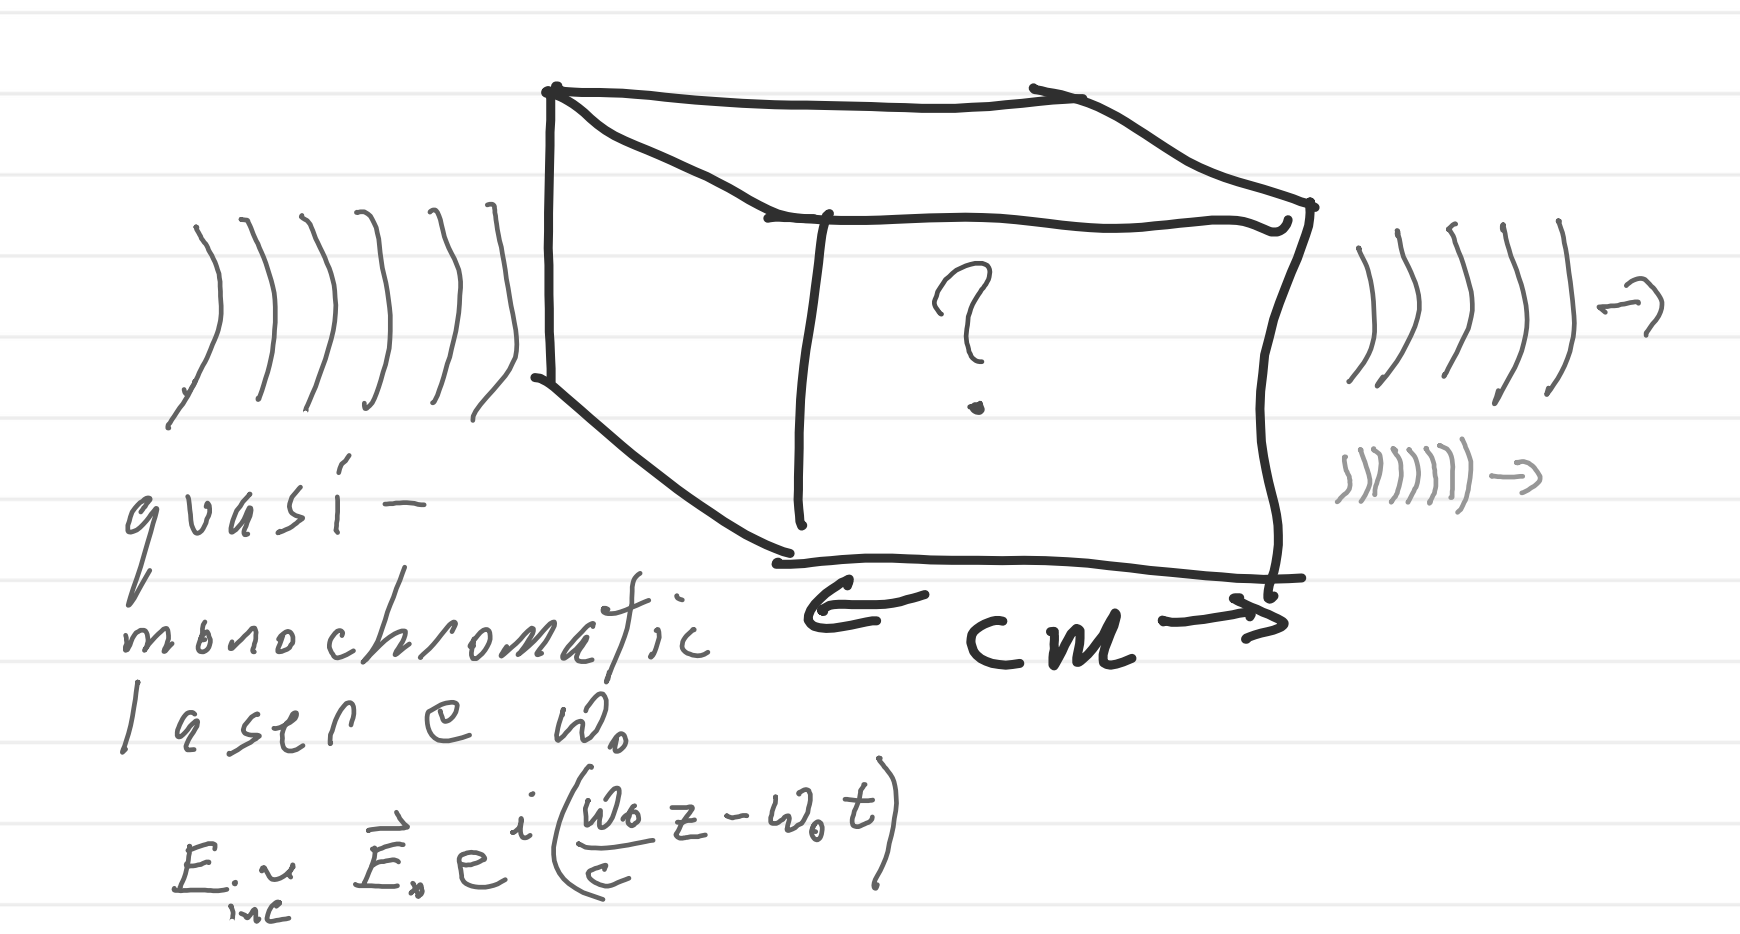
\includegraphics[width=0.6\textwidth]{figures/nonlinear_crystal.png}
    \centering
    \caption{h}
\end{figure}

\section{Heuristic linear propagation}
We will first begin with the simplest possible case of an incident wave normally-incident on a semi-infinite medium, as illustrated in Figure \ref{fig:plane_wave_normal_incidence}. The dielectric environment is invariant in the two transverse directions, and is divided into region I and region II at $z=0$. Let us assume that the incident field is a plane wave with angular frequency $\omega_{\rm{inc}}$ and free-space wavelength $\lambda_{\rm{inc}}$, and it is traveling in vacuum ($\epsilon=1$) in the positive z direction. We consider that the incident field is generated by a source that is external to our system. 

\begin{figure}
    \label{fig:plane_wave_normal_incidence}
    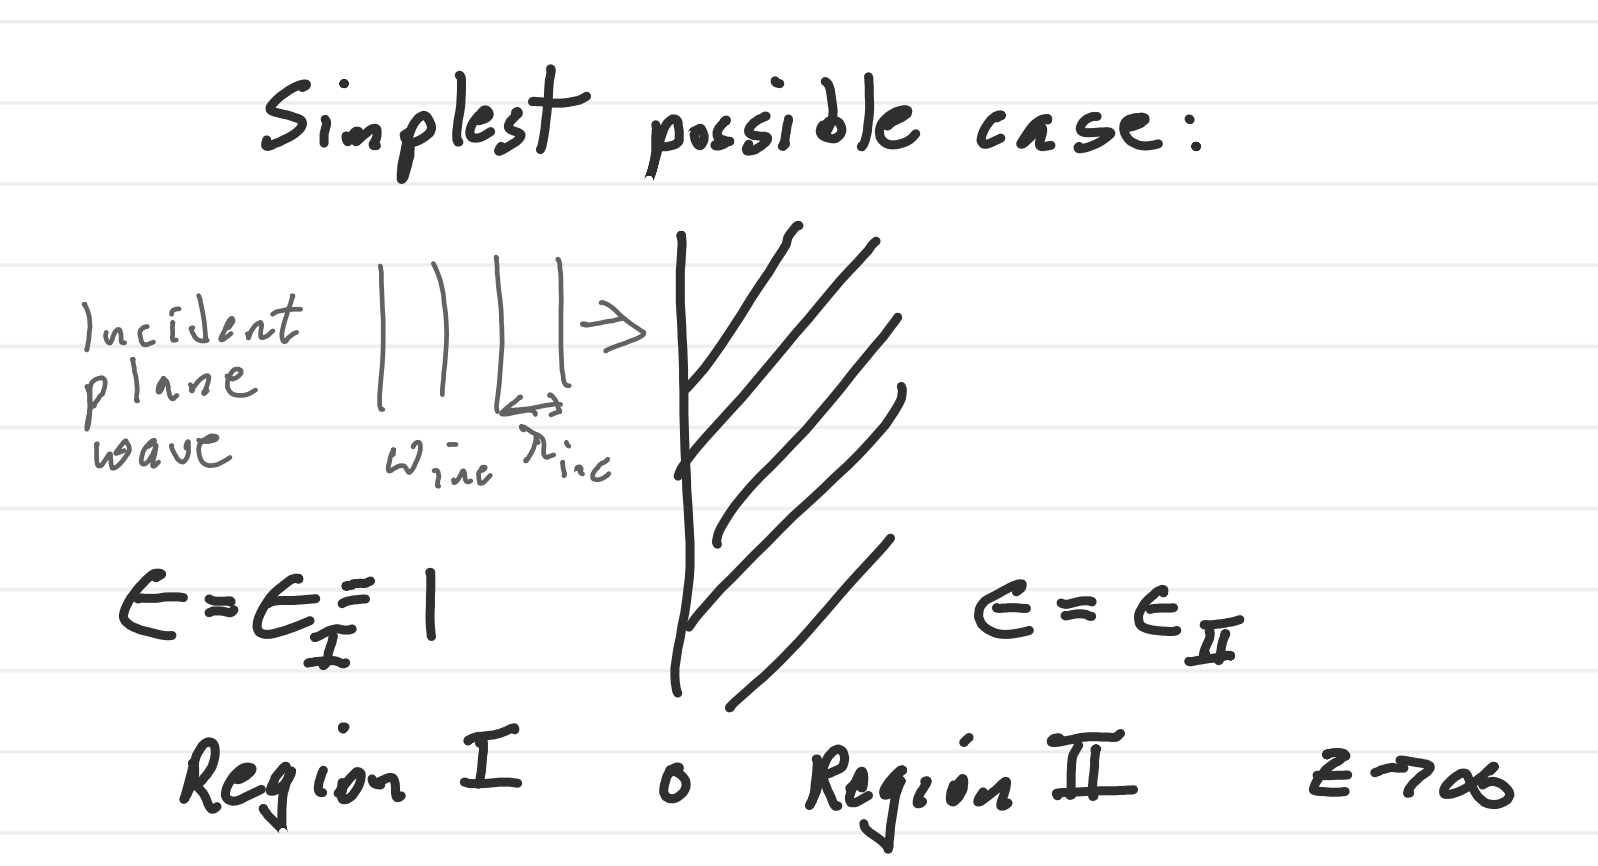
\includegraphics[width=0.6\textwidth]{figures/plane_wave_normal_incidence.png}
    \centering
    \caption{h}
\end{figure}

The main questions that we are concerned with are:
\begin{enumerate}
    \item What are the scattered fields?
    \item What is the source of the scattered fields?
\end{enumerate}

Immediately, we can give qualitative answers to these questions: There are two scattered fields: the transmitted field, and the reflected field. The source of these scattered fields is the oscillations of the electrons inside region II. We 

\subsection{Maxwell's equations}

\end{document}
